\documentclass[a4paper]{scrartcl}

\usepackage{float}
\usepackage{tikz}
\usetikzlibrary{arrows,automata}
\usepackage{pgf}
\usepackage[utf8]{inputenc} % this is needed for umlauts
\usepackage[ngerman]{babel} % this is needed for umlauts
\usepackage[T1]{fontenc}    % this is needed for correct output of umlauts in pd
\usepackage{amssymb}
\usepackage{amsmath}
\usepackage{dsfont}
\usepackage{graphicx}
\usepackage{fancyhdr}
\usepackage{lastpage}
\usepackage{imakeidx}
\setlength{\parskip}{\medskipamount}
\setlength{\parindent}{0pt}
\usepackage{enumitem}
\usepackage{hyperref}

%%%%%%%%%%%%%%%%%%%%%%%%
% Kopf- und Fusszeilen %
%%%%%%%%%%%%%%%%%%%%%%%%
\pagestyle{fancy}
\lhead{
        Maximilian Roth
}
\chead{Logik-Tutorat Lösungen Blatt 1\\}
\rhead{
        \today{} \\
        Seite \thepage{} von \pageref{LastPage}\\
        
}
\lfoot{}
\cfoot{}
\rfoot{} 

%%%%%%%%%%%%%%%%%%%%%%%%
% Anfang des Dokuments %
%%%%%%%%%%%%%%%%%%%%%%%%

\begin{document}
\section*{Disclaimer}%
\label{sec:disclaimer}
Auch in diesem Dokument können sich Fehler befinden!\\
Sie sind nicht die Musterlösung der Aufgaben, sondern selbst erstellte Lösungen.\\

Als generelle Lektüre kann ich nur das Skript von Markus Junker aus dem WS 17/18 empfehlen:\\
\url{http://home.mathematik.uni-freiburg.de/junker/skripte/InfoLogik.pdf}\\
Hier ist vieles sehr genau und verständlich erklärt.

\section*{Aufgabe 1}

Tipp1: Nutze bei solchen Aufgaben \url{http://logictools.org/} um  deine Lösung zu überprüfen.\\\\
Tipp2: Formeln mit keinem oder nur Junktoren EINES der beiden Typen: $\lor$, $\land$ sind immer in DNF sowie KNF.

Vorgehensweise:\\
\begin{itemize}
    \item Vereinfache $\rightarrow$ und $\leftrightarrow$
    \item Ziehe $\neg$ so weit hinein wie möglich
    \item Ab hier heißt es dann zielgerichtet die Formel vereinfachen\\
\end{itemize}

\begin{itemize}
    \item a)\\
        \begin{minipage}[t]{0.55\textwidth}
            Rechnung:\\
            \\
            $((P \rightarrow Q) \rightarrow (Q \rightarrow \neg R))$\\
            $\sim (\neg (P \rightarrow Q) \lor (Q \rightarrow \neg R))$\\
            $\sim (\neg (\neg P \lor Q) \lor (\neg Q \lor \neg R))$\\
            $\sim ((P \land \neg Q) \lor (\neg Q \lor \neg R))$\\
            \\
            \\
            $\sim (\neg Q \lor \neg R)$\\
        \end{minipage}
        \begin{minipage}[t]{0.4\textwidth}
            Operationen:\\
            \\
            Definition $\rightarrow$\\
            Def. $\rightarrow$\\
            Def. $\land$\\
            Distributivgesetze\\
            (Hier bereits in DNF\\
            Außen: $\lor$, Innen: $\land$)\\
            KNF und DNF

        \end{minipage}

\newpage

    \item b)\\
        \begin{minipage}[t]{0.55\textwidth}
            Rechnung:\\
            \\
            $((P \land Q) \rightarrow (P \rightarrow \neg (Q \lor R)))$\\
            $\sim (\neg (P \land Q) \lor (\neg P \lor \neg (Q \lor R)))$\\
            $\sim ((\neg P \lor \neg Q) \lor (\neg P \lor (\neg Q \land \neg R)))$\\
            \\
            $\sim ((\neg P \lor \neg Q) \lor ((\neg P \lor \neg Q) \land (\neg P \lor \neg R)))$\\
            $\sim (\neg P \lor \neg Q)$\\
        \end{minipage}
        \begin{minipage}[t]{0.4\textwidth}
            Operationen:\\
            \\
            Definition $\rightarrow$\\
            Def. $\land$\\
            Distributivgesetze\\
            (Hier bereits in DNF)\\
            Vereinfachen\\
            KNF und DNF
        \end{minipage}
\end{itemize}

\section*{Aufgabe 2}%
\label{sec:aufgabe_2}

Tipp:\\
Fange hier mit der "unübersichtlichen" Gleichung an und vereinfache sie.\\
Oder vereinfache direkt beide, falls sie unübersichtlich sind.

        \begin{minipage}[t]{0.55\textwidth}
            Rechnung:\\
            \\
            $(P \rightarrow (Q \rightarrow R))$\\
            $\sim (\neg P \lor (\neg Q \lor R))$\\
            $\sim ((\neg P \lor \neg Q) \lor R)$\\
            $\sim (\neg (P \land Q) \lor R)$\\
            $\sim ((P \land Q) \rightarrow R)$\\
        \end{minipage}
        \begin{minipage}[t]{0.4\textwidth}
            Operationen:\\
            \\
            Definition $\rightarrow$\\
            Mit Blick auf Lösung umstellen\\
            Def. $\land$\\
            Def. $\rightarrow$
        \end{minipage}

\newpage

\section*{Aufgabe 3}%
\label{sec:aufgabe_3}

Tipp1:\\
Schaue Dir zuerst die Formel an und überlege dir, ob sie eine Tautologie ist und falls nein, woran es scheitert.
Entwerfe erst danach deinen Baum.\\
\\
Tipp2:\\
Überprüfe deine Lösung mit einem der folgenden Tools:\\
\url{http://www.formallogic.com/en/truth-tree-solver}\\
\url{https://www.umsu.de/logik/trees/}\\
\url{http://www.gablab.net/truth-tree-solver/sentential-logic}\\
\\
Vorgehensweise:\\
Da wir zeigen müssen, dass die Formeln Tautologien sind versuchen wir Belegungen zu finden, die die Formel zu Falsch evaluieren lassen.\\
Siehe auch die Anleitung auf der letzten Seite an.


\begin{itemize}
    \item a)\\

        Alle Zweige schließen, da sie in einer Belegung eine ältere überschreiben würden.\\
        $\Rightarrow$ Es ist nicht möglich, dass die Formel Falsch wird.\\
        $\Leftrightarrow$ Die Formel ist eine Tautologien.

        \begin{figure}[H]
            \centering
            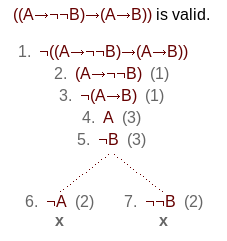
\includegraphics[scale=0.6]{3-a-tree.png}
            \caption{Lösung zu 3 a)}
            \label{fig:}
        \end{figure}

\newpage

    \item b)\\

        Es gibt Zweige die nicht schließen.\\
        $\Rightarrow$Die Formel kann falsch werden mit:\\
        $P \sim \top, Q \sim \bot$

        \begin{figure}[H]
            \centering
            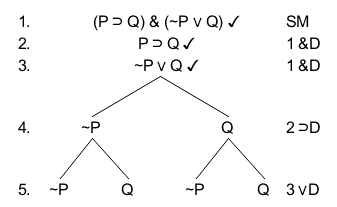
\includegraphics[scale=0.6]{3-b-tree.png}
            \caption{Lösung zu 3 b)}
            \label{fig:name}
        \end{figure}

    \item c)\\

        Diese Formel wurde von $A_1,...,A_k$ zu A,B,... umbenannt under der Einfachheit halber auf A-D reduziert, die Art des Beweises bleibt jedoch gleich (wird jedoch übersichtlicher).\\
        Um zu sehen, wie ein Beweis mit beliebigem k aussieht siehe e).\\
        Alle Zweige schließen $\Rightarrow$ Tautologie\\

        \begin{figure}[H]
            \centering
            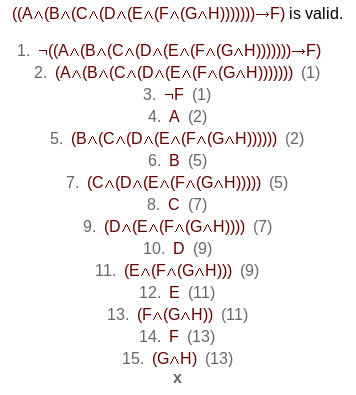
\includegraphics[scale=0.49]{3-c-tree.png}
            \caption{Lösung zu 3 c)}
            \label{fig:name}
        \end{figure}

    \item d)\\

        Alle Zweige schließen, da sie alte Werte überschreiben würden.\\
        $\Rightarrow$ Die Formel ist Tautologie.

        \begin{figure}[H]
            \centering
            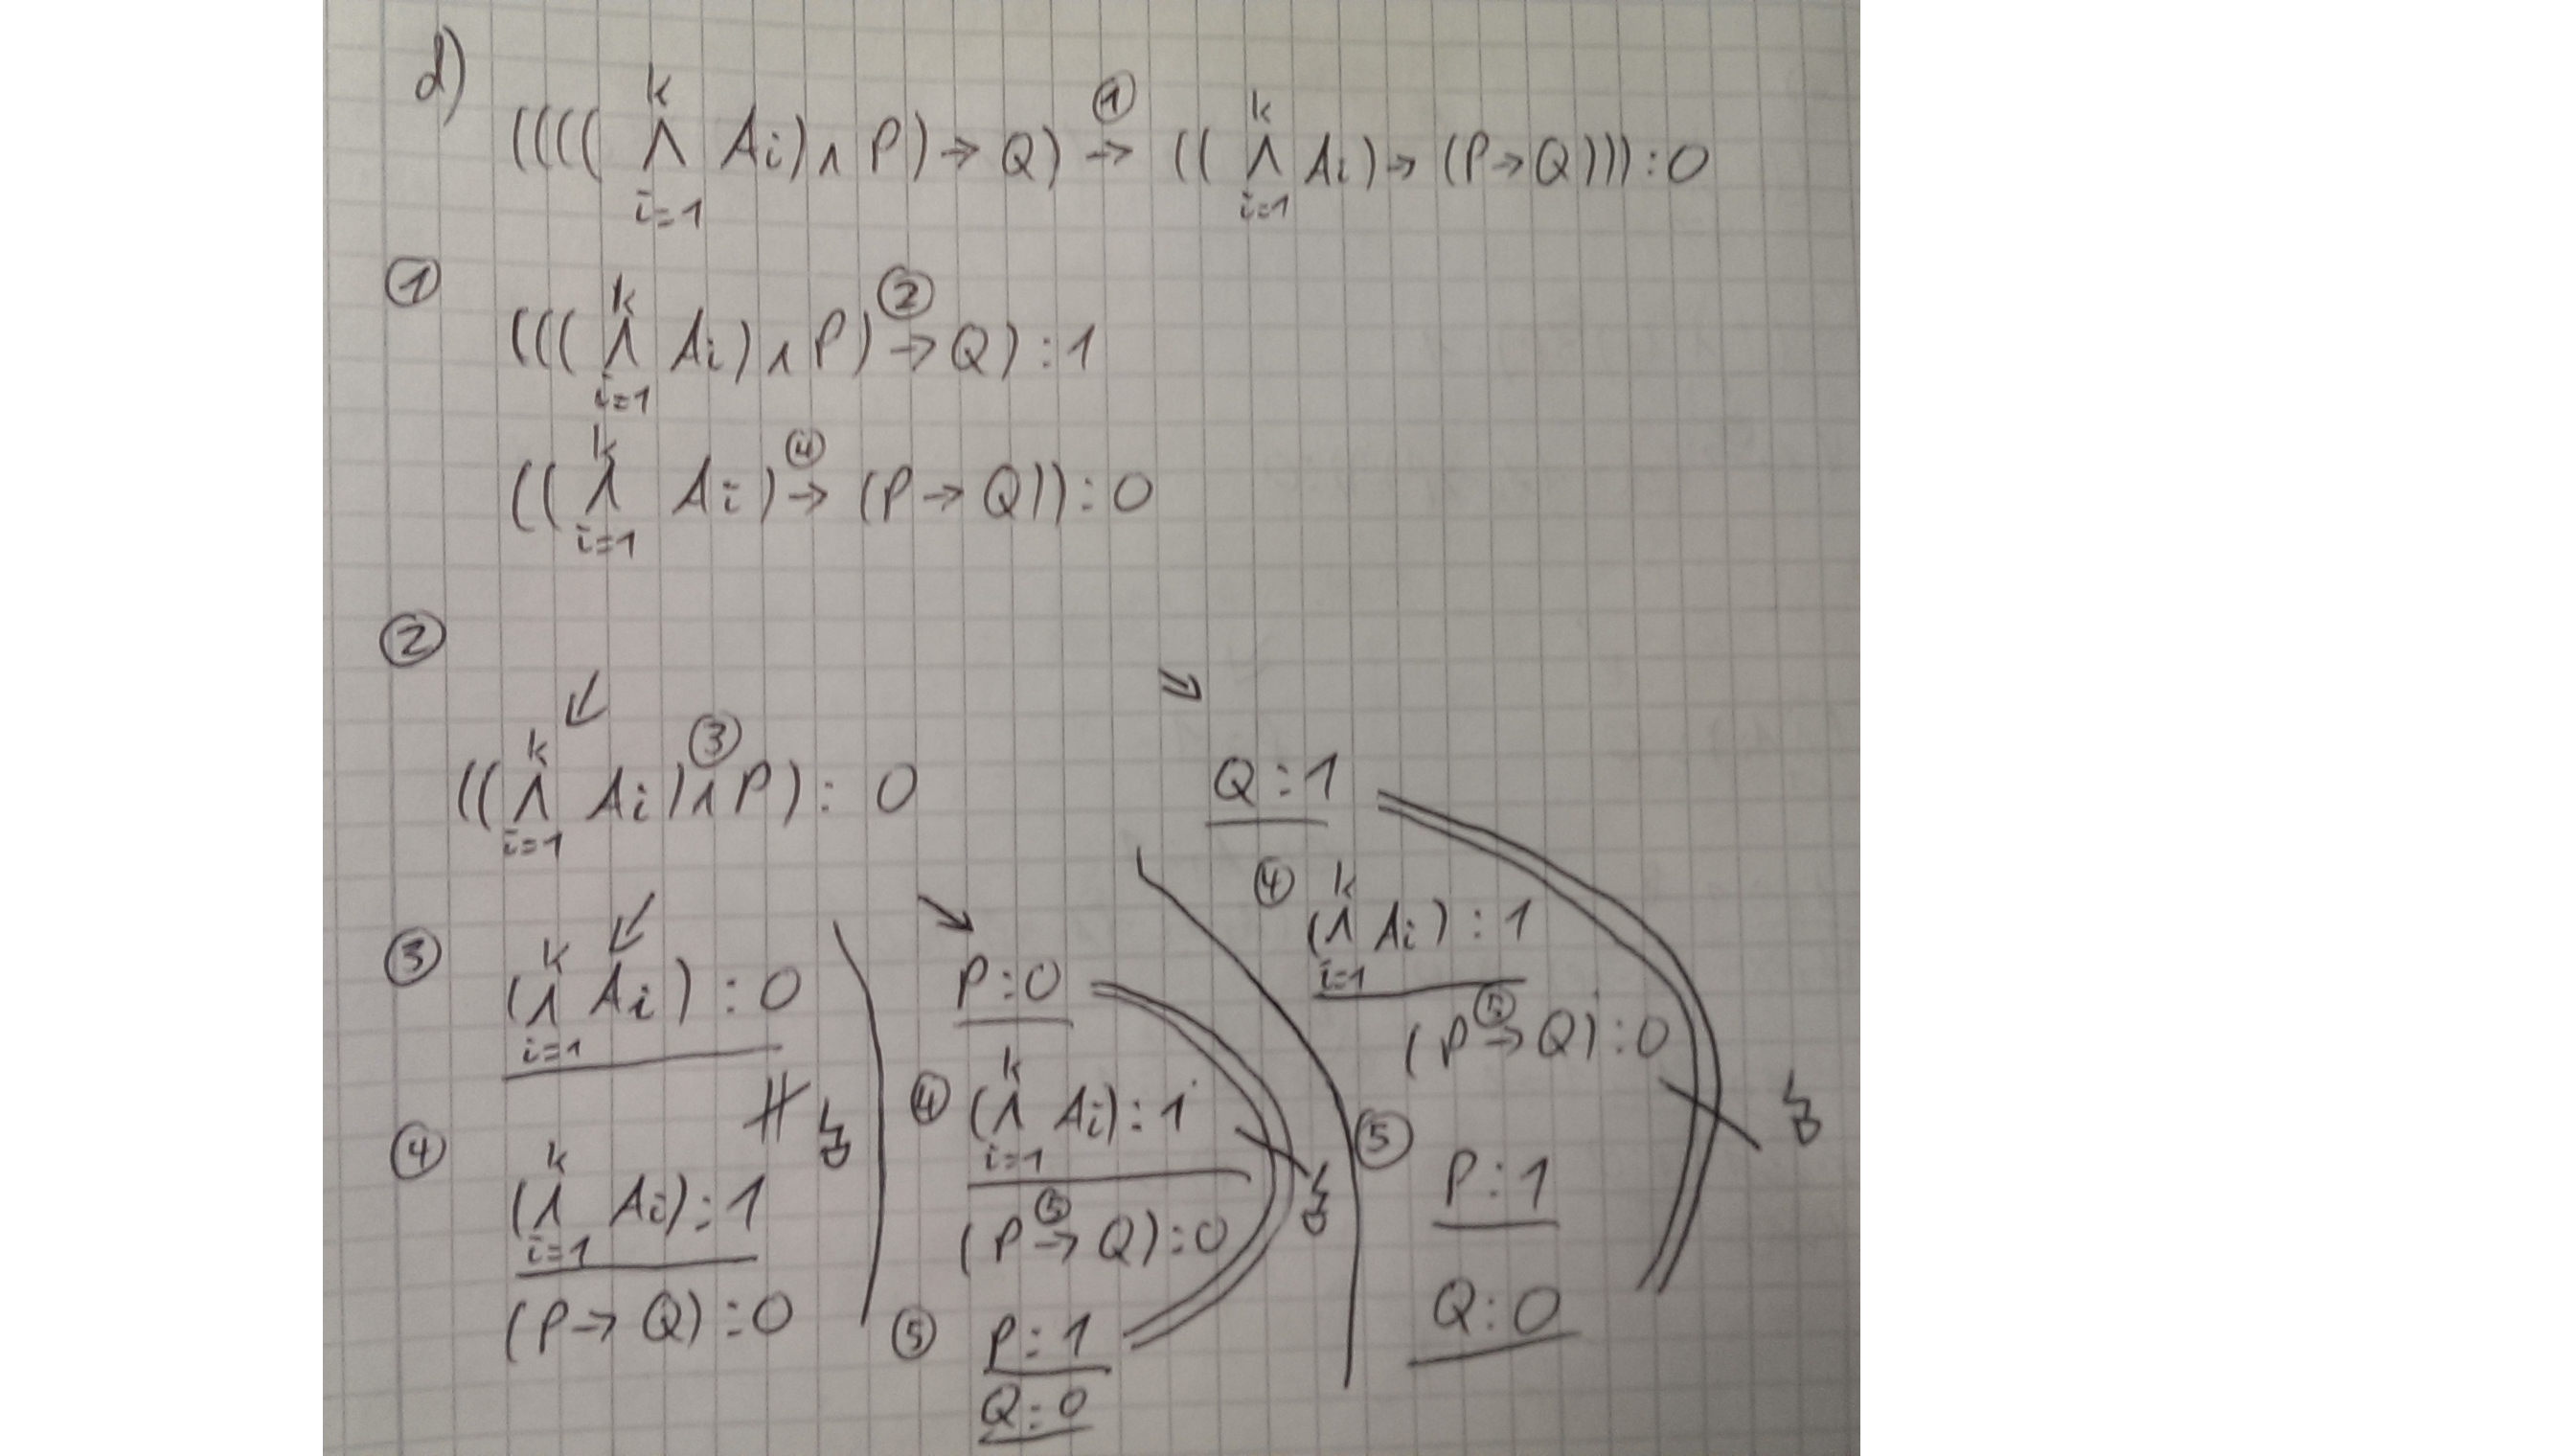
\includegraphics[scale=0.25]{3-d-tree.png}
            \caption{Lösung zu 3 d)}
            \label{fig:name}
        \end{figure}

\newpage

    \item e)\\

        Für alle Zwischenschritte gilt: $A_x$ muss wahr sein und alles rechts in der Formel muss \textbf{Als ganzes, d.h. nicht unbedingt alle Teile} falsch sein.\\
        Alle Zweige schließen, da sie alte Werte überschreiben würden.\\
        $\Rightarrow$ Die Formel ist Tautologie.

        \begin{figure}[H]
            \centering
            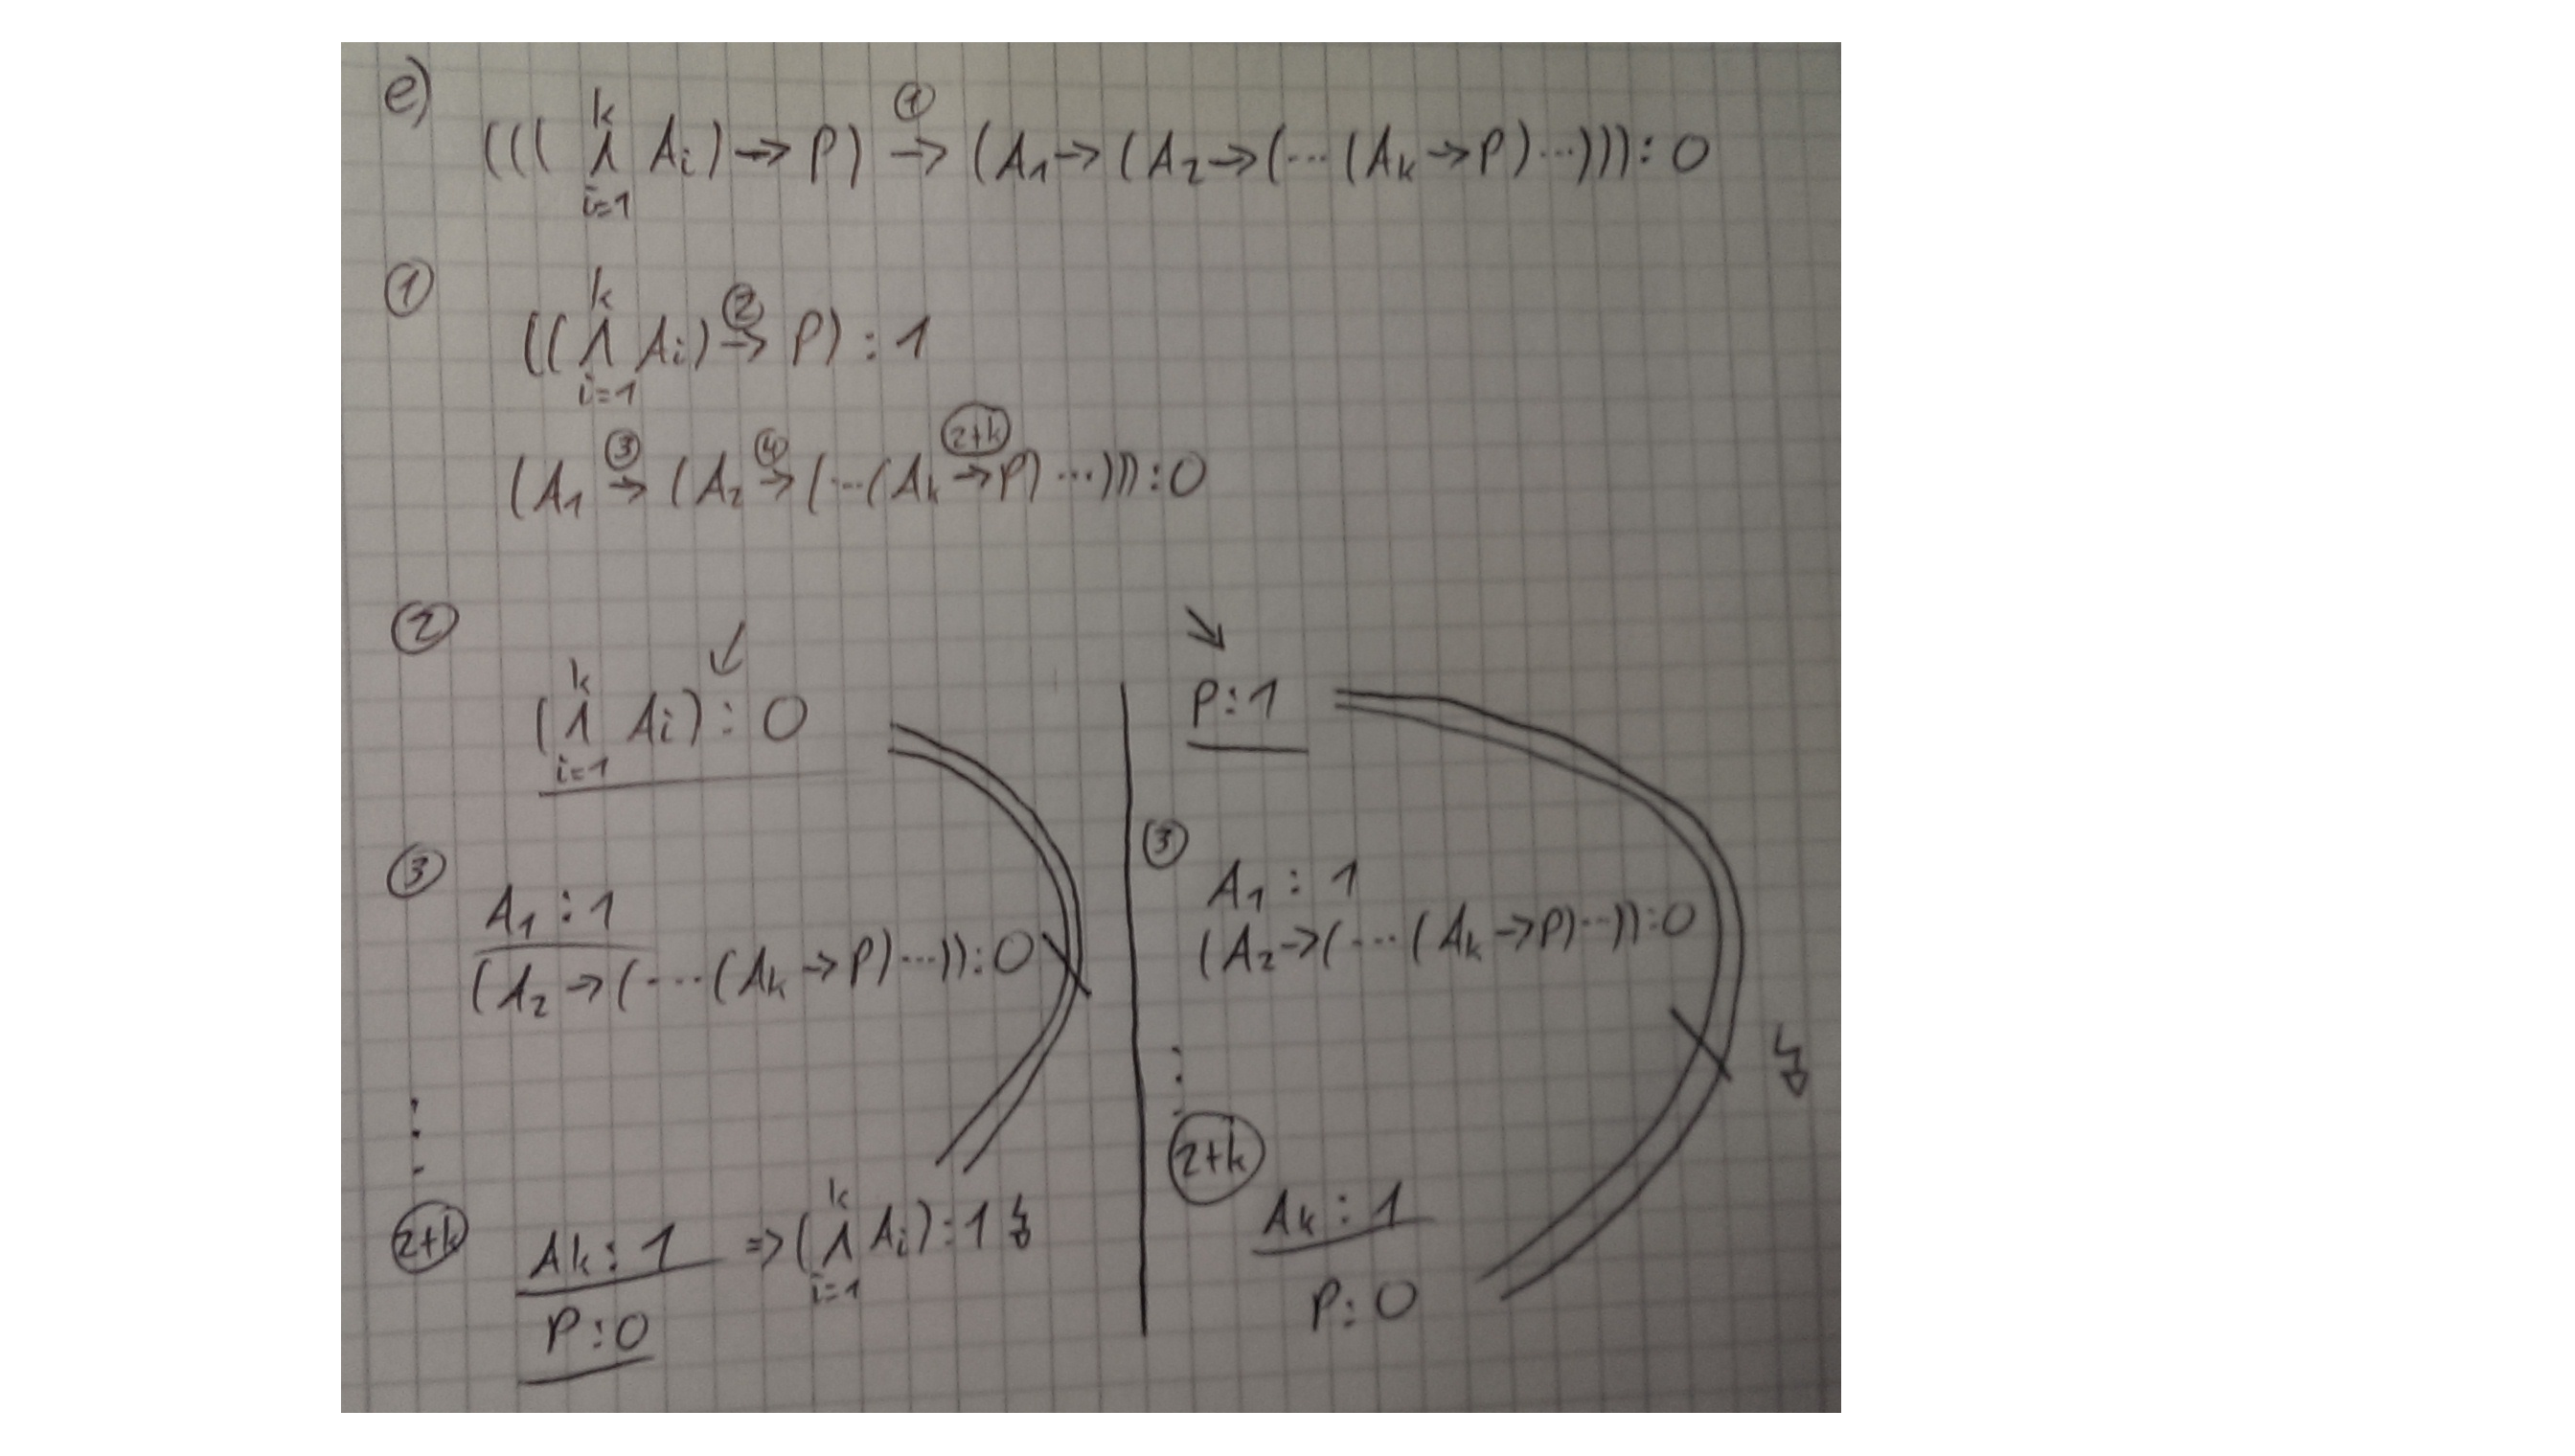
\includegraphics[scale=0.25]{3-e-tree.png}
            \caption{Lösung zu 3 e)}
            \label{fig:name}
        \end{figure}
\end{itemize}

\newpage

\section*{Aufgabe 4}%
\label{sec:aufgabe_4}

\begin{itemize}
    \item a)\\
        \underline{ZZ:} $E^\mathfrak{B}$ ist Äquivalenzrelation auf F(A) $\subseteq$ B.\\
        \underline{Bew:}\\
        \\Wir zeigen die Eigenschaften einer Äquivalenzrelation: Reflexivität, Symmetrie, Transitivität.
        \begin{itemize}
            \item i) \underline{Reflexivität:}\\
                Sei $b \in F(A) \overset{\text{f inj.}}{\Rightarrow} \overset{!}{\exists} a \in A: F(a) = b$\\
                $\Rightarrow (a,a)\in E^\mathfrak{A}$\\
                \\$\overset{\text{starker }\mathfrak{L}\text{-Hom.}}{\Leftrightarrow} (F(a),F(a)) \in E^\mathfrak{B}$\\
                $\Leftrightarrow (b,b)\in E^\mathfrak{B}$\\
                \\Dies gilt immer, da $E^\mathfrak{A}$ Äquivalenzrelation ist. $\Rightarrow E^\mathfrak{B}$ ist reflexiv.\\
            \item ii) \underline{Symmetrie:}\\
                Seien $b_1, b_2 \in F(A)$\\
                $\Rightarrow \overset{!}{\exists} a_1 \in A: F(a_1) = b_1$\\
                $\Rightarrow \overset{!}{\exists} a_2 \in A: F(a_2) = b_2$\\
                \\Dann gilt $(b_1,b_2) \in E^\mathfrak{B}$\\
                $\Leftrightarrow (F(a_1),F(a_2)) \in E^\mathfrak{B}$\\
                $\overset{\text{starker }\mathfrak{L}\text{-Hom.}}{\Leftrightarrow} (a_1,a_2) \in E^\mathfrak{A}$\\
                $\overset{E^\mathfrak{A} \text{ Äquivrel.}}{\Leftrightarrow} (a_2,a_1) \in E^\mathfrak{A}$\\
                $\Leftrightarrow (F(a_2),F(a_1)) \in E^\mathfrak{B}$\\
                $\Leftrightarrow (b_2,b_1) \in E^\mathfrak{B}$\\
                \\$\Rightarrow E^\mathfrak{B}$ ist symmetrisch.\\

\newpage

            \item iii) \underline{Transitivität:}\\
                Seien $b_1,b_2,b_3 \in F(A)$\\
                $\Rightarrow \overset{!}{\exists} a_1 \in A: F(a_1) = b_1$\\
                $\Rightarrow \overset{!}{\exists} a_2 \in A: F(a_2) = b_2$\\
                $\Rightarrow \overset{!}{\exists} a_3 \in A: F(a_3) = b_3$\\
                \\Und gelte: $(a_1,a_2) \in E^\mathfrak{A}, (a_2,a_3) \in E^\mathfrak{A}$\\
                $\Rightarrow (b_1,b_2) \in E^\mathfrak{B}$ und $(b_2,b_3) \in E^\mathfrak{B}$\\
                $\Leftrightarrow (F(a_1),F(a_2)) \in E^\mathfrak{B}$ und $(F(a_2),F(a_3)) \in E^\mathfrak{B}$\\
                $\overset{\text{starker }\mathfrak{L}\text{-Hom.}}{\Leftrightarrow} (a_1,a_2) \in E^\mathfrak{A}$ und $(a_2,a_3) \in E^\mathfrak{A}$\\
                $\overset{E^\mathfrak{A} \text{ Äquivrel.}}{ \underline{\Rightarrow}} (a_1,a_3)\in E^\mathfrak{A}$\\
                $\overset{\text{starker }\mathfrak{L}\text{-Hom.}}{\Leftrightarrow} (F(a_1),F(a_3)) \in E^\mathfrak{B}$\\
                $\Leftrightarrow (b_1,b_3) \in E^\mathfrak{B}$\\
                $\Rightarrow E^\mathfrak{B}$ ist transitiv.\\

        \end{itemize}
    \item b)\\
        \underline{ZZ:} $\mathfrak{A}$ und $\mathfrak{B}$ lassen sich jeweils ineinander einbetten.\\
        \underline{Bew:}\\
        Für eine Einbettung sind eine injektive Abbildung F und folgende Eigenschaften notwendig:\\

        \begin{figure}[H]
            \centering
            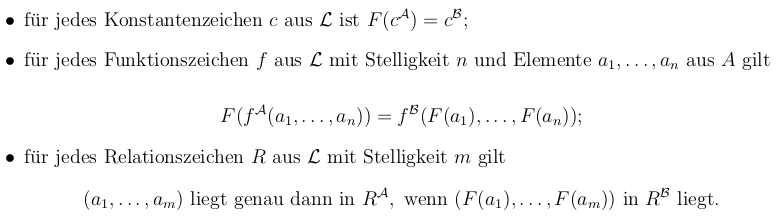
\includegraphics[scale=0.6]{Def-Einbettung.png}
            \caption{Eigenschaften Einbettung}
            \label{fig:}
        \end{figure}

\newpage

        \begin{itemize}
            \item i)\\
                Wir definieren die Abbildung F, die von A = \{$a_0,a_1\} \cup \{a_{i,j} | i,j \in \mathds{N}$\}\\
                nach B = \{$b_0, b_1, b_2, b_3\} \cup \{b_{i,j} | i,j \in \mathds{N}\}$ abbildet.\\
                \\Weiter definieren wir die Äquivalenzklassen:\\
                Für A:\\
                $[a_0]_{A^\mathfrak{A}} = \{a_0,a_1\}$\\
                $[a_{i,j}]_{A^\mathfrak{A}} = \{a_{i,k} | k \in \mathds{N}\}$\\
                \\Für B:\\
                $[b_0]_{A^\mathfrak{B}} = \{b_0,b_1\}$\\
                $[b_2]_{A^\mathfrak{B}} = \{b_2,b_3\}$\\
                $[b_{i,j}]_{A^\mathfrak{B}} = \{b_{i,k} | k \in \mathds{N}\}$\\
                \\F bildet die Elemente von A nach B wie folgt ab:\\
                $a_0 \mapsto b_0$\\
                $a_1 \mapsto b_1$\\
                $a_{ij} \mapsto b_{ij}, \forall i,j \in \mathds{N}$\\
                \\F ist injektiv, da keine zwei a existieren, die auf das selbe b abbilden.\\
                F erfüllt die ersten beiden weiteren Eigenschaften, da die \mathfrak{L}-Struktur weder Konstanten noch Funktionen besitzt.\\
                Durch nachprüfen lässt sich leicht feststellen, dass auch die 3. Eigenschaft gilt.\\

            \item ii)\\
                A und B seien wie oben definiert, ebenso die Äquivalenzklassen.\\
                Wir definieren also nur eine neue Abbildung G, die wie folgt abbildet:\\
                \\$b_0 \mapsto a_0$\\
                $b_1 \mapsto a_1$\\
                $b_2 \mapsto a_{0,0}$\\
                $b_3 \mapsto a_{0,1}$\\
                $b_{i,j} \mapsto a_{i+1,j}$\\
                \\Wieder gelten die Eigenschaften 1 und 2 trivialerweise und auch Eigenschaft 3 gilt offensichtlich.\\



        \end{itemize}

        \underline{ZZ:} $\mathfrak{A}$ und $\mathfrak{B}$ sind nicht Isomorph.\\
        \underline{Bew:}\\
        \\Die Tatsache, dass $\mathfrak{B}$ zwei Äquivalenzklassen besitzt, aber $\mathfrak{A}$ nur eine macht einen Isomorphismus unmöglich,
        da für ihn auch surjektivität nötig ist,\\
        aber wir bei i) gar nicht auf $b_2, b_3$ abbilden.

\end{itemize}

\newpage

\section*{Anmerkung: Baumkalkül / Tableaumethode}%
\label{sec:anmerkung_baumkalkul_tableaumethode}
    Quelle beider Bilder: Skript "Logik für Informatiker" Markus Junker WS 17/18:\\
    \url{http://home.mathematik.uni-freiburg.de/junker/skripte/InfoLogik.pdf}\\

    Eigentlich recht einfach im Prinzip, jedoch recht langwierig in der Praxis.\\
    Man legt erst fest, ob eine Formel wahr oder falsch "gemacht" werden soll und teilt dann die Formel dementsprechen in Subteile auf, wie auf folgender Graphik erklärt:

    \begin{figure}[H]
        \centering
        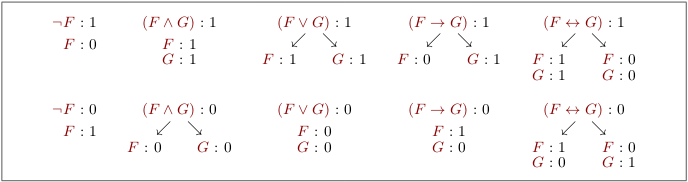
\includegraphics[scale=0.6]{Baumkalkuel.png}
        \caption{Aufteilungen}
        \label{fig:}
    \end{figure}

    Und dazu noch ein Beispiel. Hier wäre es möglicherweise cleverer gewesen zu zeigen, dass es keine Tautologie ist, statt anzunehmen, dass es keine ist und dann durch Zufall ein Gegenbeispiel zu finden.

    \begin{figure}[H]
        \centering
        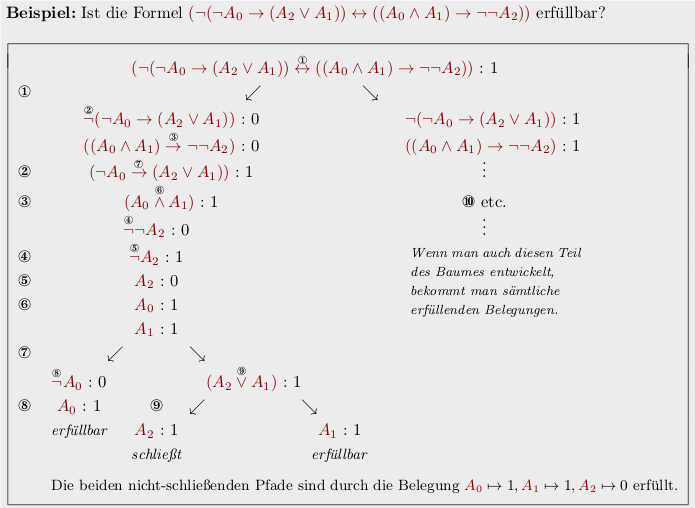
\includegraphics[width=0.8\textwidth, height=0.34\textheight]{Baumkalkuel-2.png}
        \caption{Beispiel}
        \label{fig:}
    \end{figure}

\end{document}
